\documentclass{article}
\usepackage{graphicx}
\usepackage[margin=1in]{geometry}
\usepackage[usenames, dvipsnames]{color}

% %
% \makeatletter
% \setlength{\@fptop}{0pt}
% \makeatother
% %

\begin{document}

\title{Supplementary material for ``Visualization methods for RNA-sequencing data analysis"}
\author{Lindsay Rutter}

\maketitle

This file contains supplementary analyses that the reader might find useful, and that extend upon several of the main concepts discussed in the paper. This supplementary document provides additional examples of parallel coordinate plots, scatterplots matrices, and litre plots, and how these plotting tools can be used to assess normalization and DEG calls. Also included are examples of the effect of standardizing data before viewing them in scatterplot matrices and litre plots.

\begin{itemize}

\item Figure~\ref{sbIRClusters} shows parallel coordinate plots of hierarchical clusters in a similar manner as Figure 2 in the main paper. The data comes from the iron-metabolism soybean study, and has been filtered and standardized. However, unlike Figure 2 in the main paper that only showed significant genes, Figure~\ref{sbIRClusters} in this supplementary file shows all genes.

\item Figure~\ref{sbIRClusterSigSM1} through Figure~\ref{sbIRClusterSigSM4} show scatterplot matrices of the significant genes in the iron-metabolism soybean dataset for each of the four clusters that resulted from hiearchical clustering analysis. They provide an additional and complementary perspective on these DEG calls from what we saw with the parallel coordinate plots in Figure~\ref{sbIRClusters}. 

\item Figure~\ref{mdsSwitch} shows that some of the most popular RNA-seq visualization tools cannot always detect common errors, such as sample switching. Side-by-side boxplots and MDS plots are shown for the soybean cotyledon dataset after deliberately switching samples between treatment groups. For the most part, they are unable to detect the error. In contrast, the less-popular method of scatterplot matrices can quickly detect the possibility of the error (see Figure 5 from the main paper).

\item Figure~\ref{litreCluster1} shows example litre plots for two significant genes from Cluster 1. The reader may wish to view it alongside Figure 8 from the main paper, which contains example litre plots for significant genes from Clusters 2, 3, and 4.

\end{itemize}


%%%%%%%%%%%%%%%%%%%%%%%%%%%%%
%%%%%%%%%%%%%%%%%%%%%%%%%%%%%
%%%%%%% Begin Figures %%%%%%% 

\clearpage
\null
\begin{figure}[t!]
\centerline{\includegraphics[width=\columnwidth]{../MakeFigures/sbIRClusters.jpg}}
\caption{Example application of parallel coordinate plots using the iron-metabolism soybean dataset. We filtered genes with low means and/or variance, performed a hierarchical clustering analysis with a cluster size of four, and visualized the results using parallel coordinate lines. Most non-filtered genes were in Clusters 1 and 2, which both showed overexpression in one treatment and underexpression in the other treatment. The genes in Cluster 4 mostly showed messy patterns with low signal to noise ratios. Interestingly, Cluster looked similar to Cluster 2 (large values for group N and small values for group P), except for unexpectedly large values for the third replicate of group P.
\label{sbIRClusters}}
\end{figure}

\clearpage
\null
\begin{figure}[t!]
\centerline{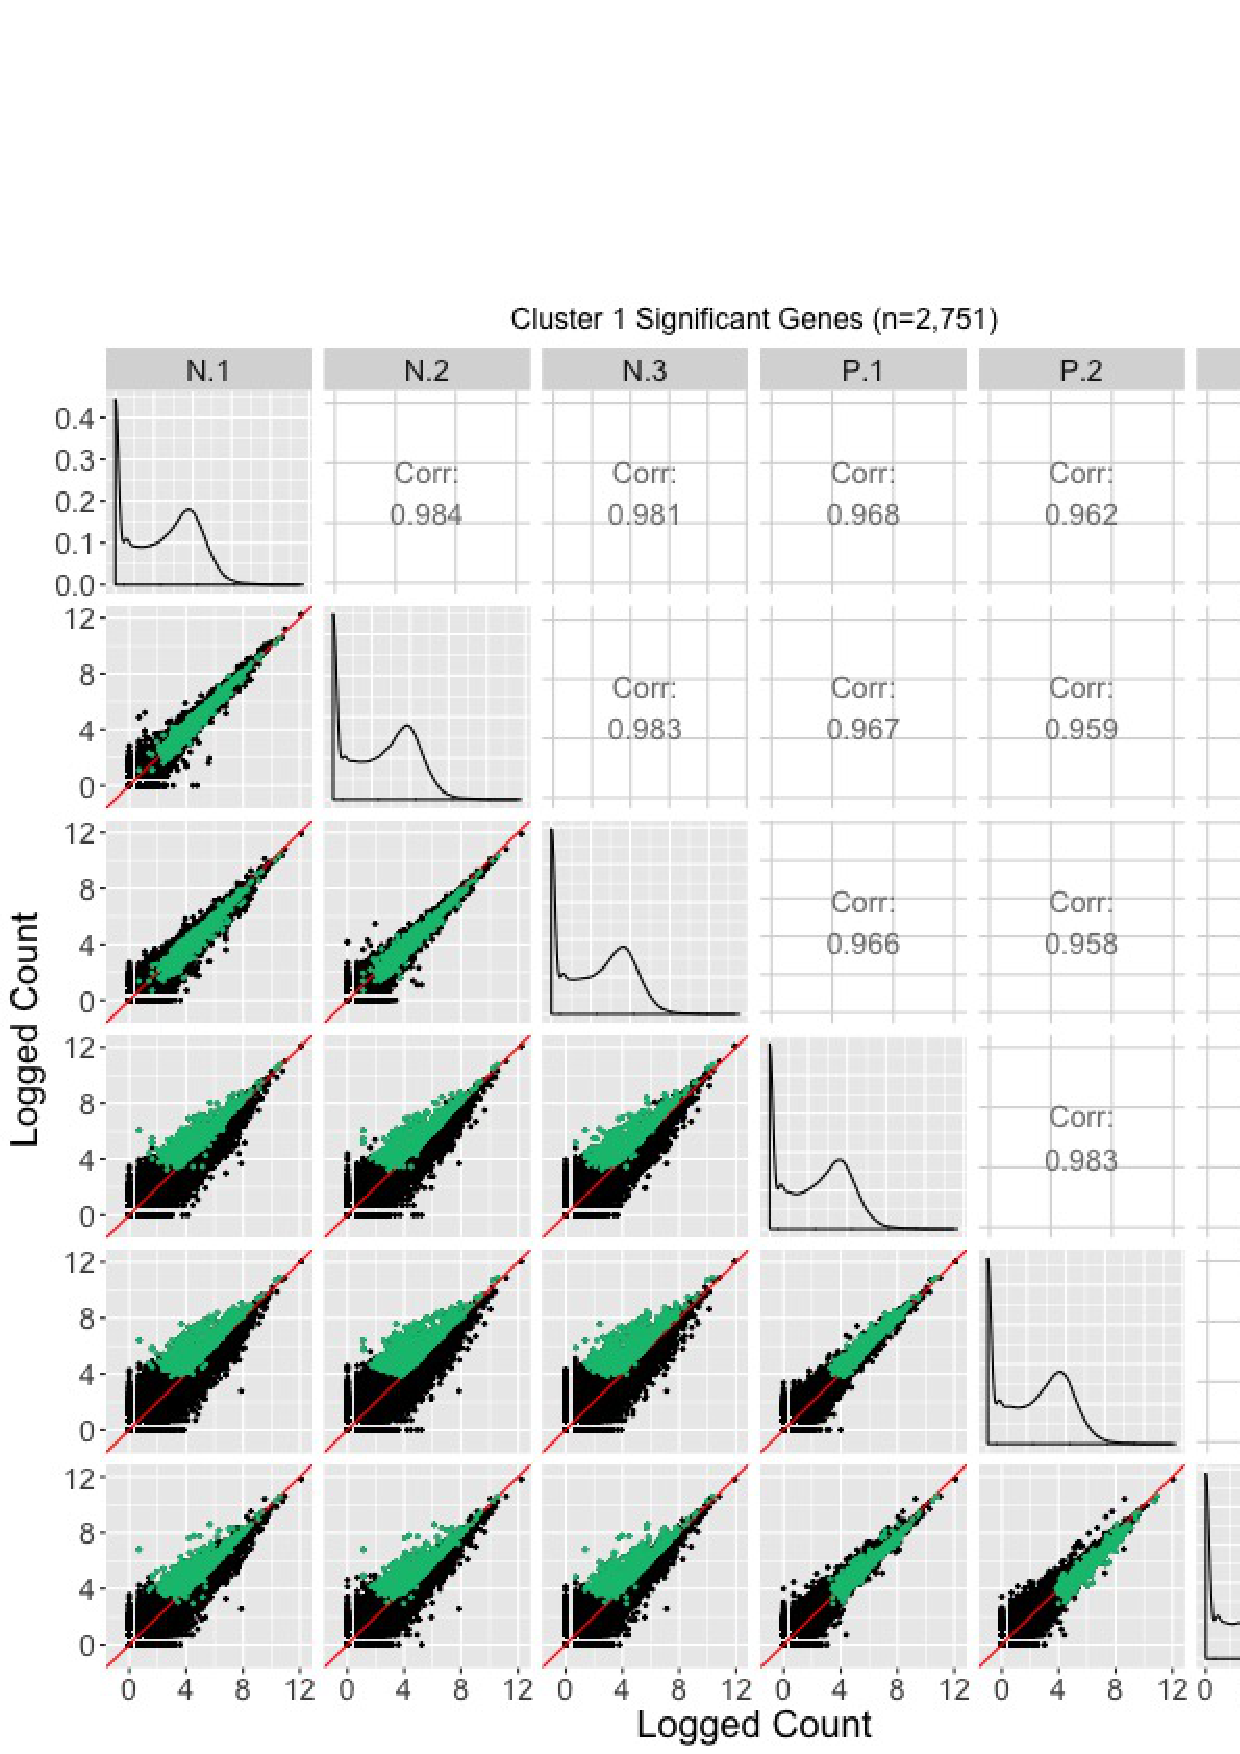
\includegraphics[width=\columnwidth]{../MakeFigures/sbIRClusterSigSM1.jpg}}
\caption{Example of using a scatterplot matrix to assess DEG calls from a model in the iron-metabolism soybean dataset. There were 2751 significant genes in Cluster 1 after performing a hierarchical clustering analysis with a cluster size of four. These significant genes are overlaid in green over the scatterplot matrix. They follow the expected patterns of differential expression with most green points falling along the \textit{x=y} line in the scatterplots between replicates, but deviating from the \textit{x=y} line in the scatterplots between treatments. The deviation consistently demonstrates higher expression in the P group than in the N group. Hence, these green points seem to represent genes that were significantly overexpressed in the P group, which draws the same conclusion with what we derived using the parallel coordinate plots in Figure 2 of the paper. One difficulty with plotting such a large number of DEGs onto the scatterplot matrix is that overplotting can obscure our inability to determine how many DEGs are in a given location.
\label{sbIRClusterSigSM1}}
\end{figure}

\clearpage
\null
\begin{figure}[t!]
\centerline{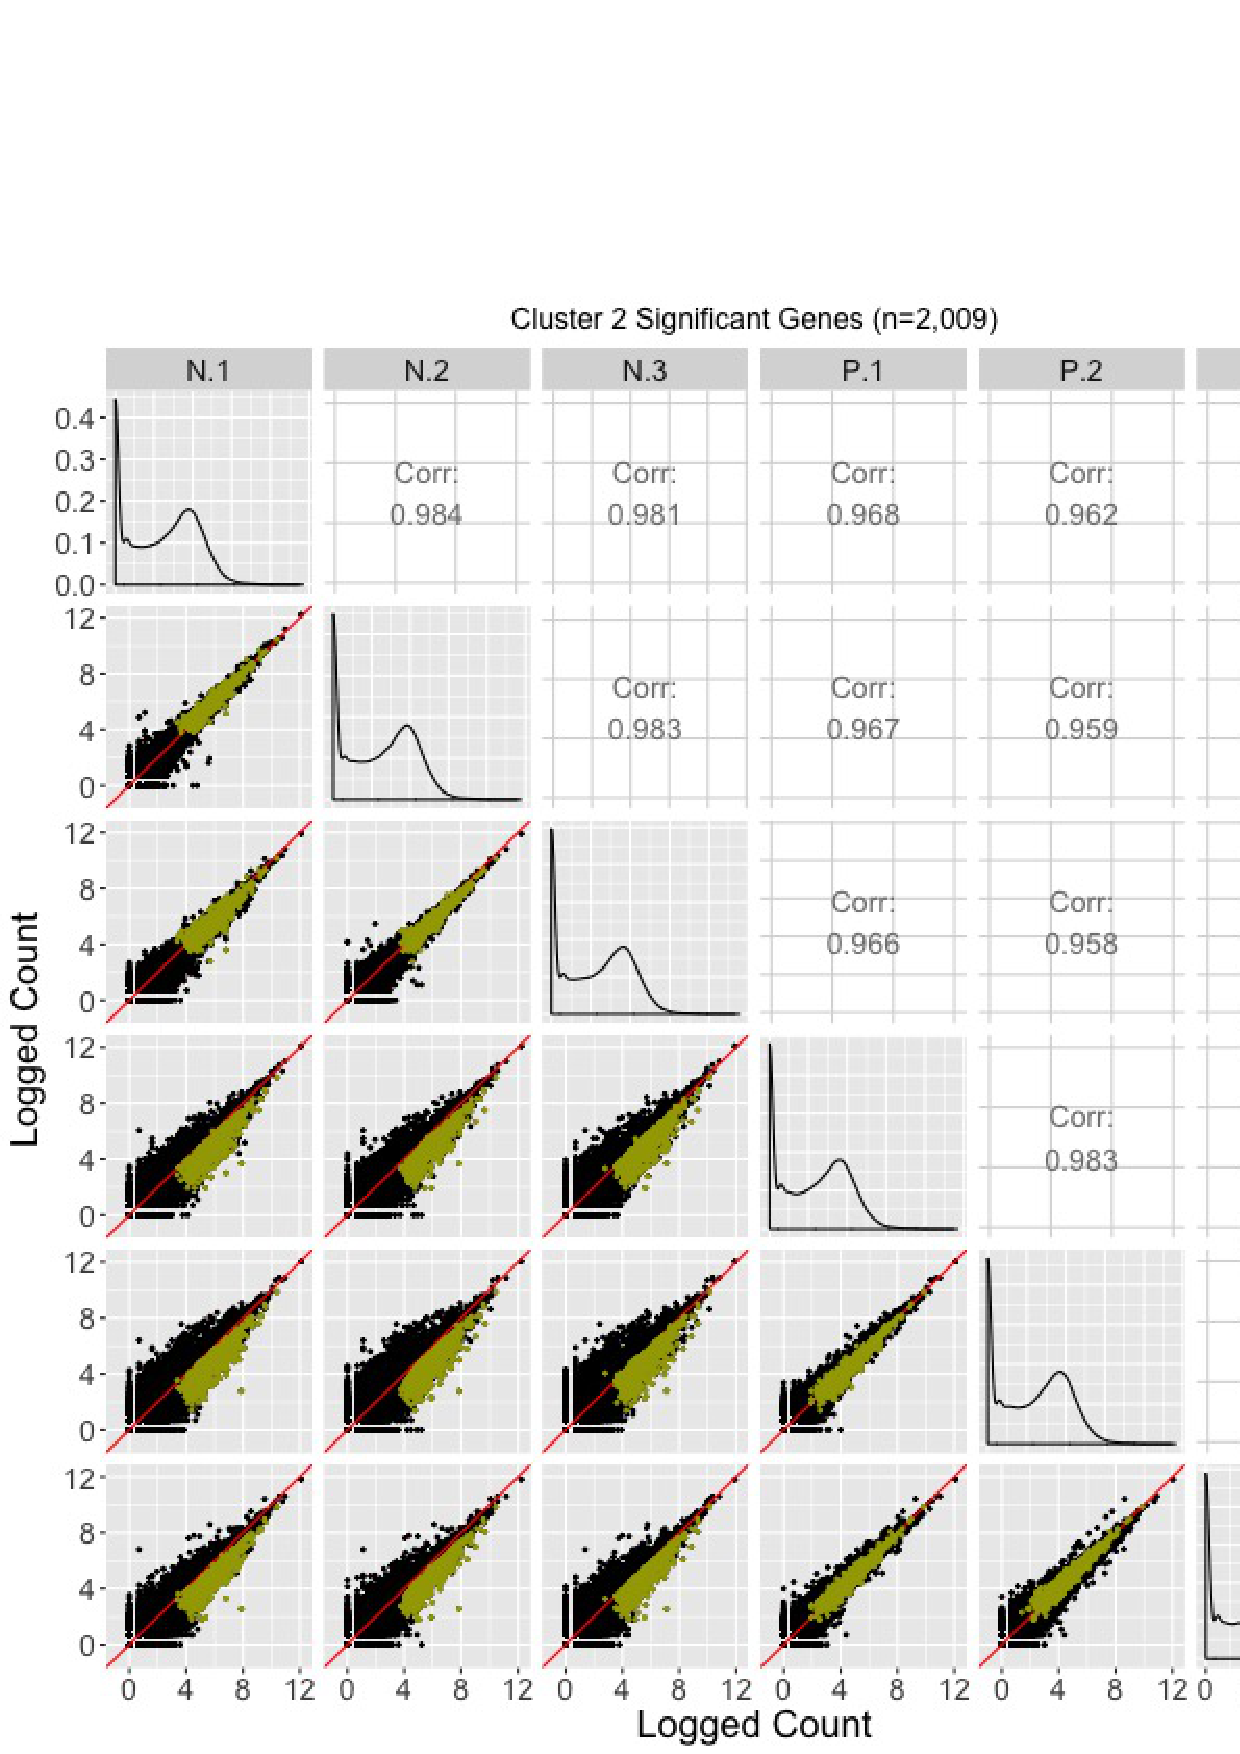
\includegraphics[width=\columnwidth]{../MakeFigures/sbIRClusterSigSM2.jpg}}
\caption{Example of using a scatterplot matrix to assess DEG calls from a model in the iron-metabolism soybean dataset. There were 2009 significant genes in Cluster 2 after performing a hierarchical clustering analysis with a cluster size of four. These significant genes are overlaid in mustard over the scatterplot matrix. They follow the expected patterns of differential expression with most mustard points falling along the \textit{x=y} line in the scatterplots between replicates, but deviating from the \textit{x=y} line in the scatterplots between treatments. The deviation consistently demonstrates higher expression in the N group than in the P group. Hence, these mustard points seem to represent genes that were significantly overexpressed in the N group, which draws the same conclusion with what we derived using the parallel coordinate plots in Figure 2 of the paper. One difficulty with plotting such a large number of DEGs onto the scatterplot matrix is that overplotting can obscure our inability to determine how many DEGs are in a given location.
\label{sbIRClusterSigSM2}}
\end{figure}
  
\null
\begin{figure}[t!]
\centerline{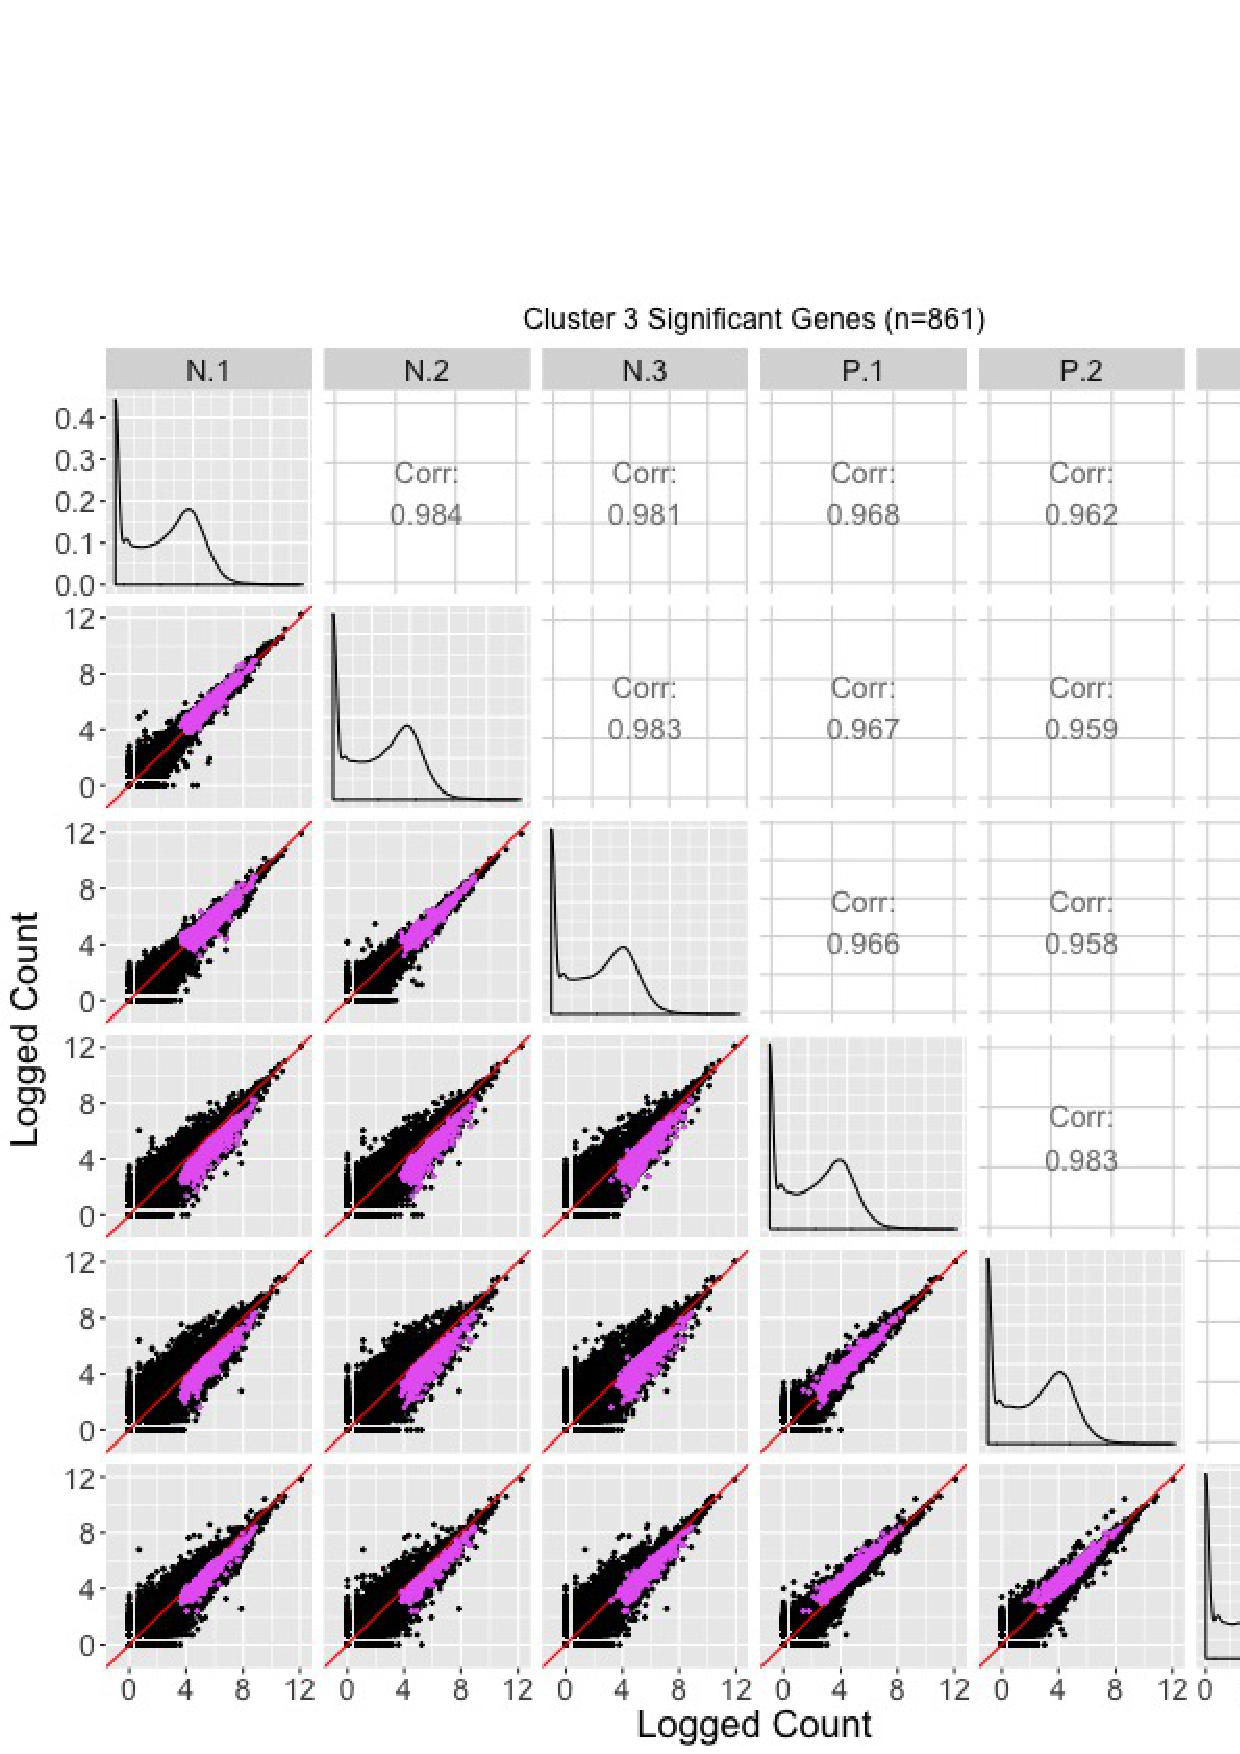
\includegraphics[width=\columnwidth]{../MakeFigures/sbIRClusterSigSM3.jpg}}
\caption{Example of using a scatterplot matrix to assess DEG calls from a model in the iron-metabolism soybean dataset. There were 861 significant genes in Cluster 3 after performing a hierarchical clustering analysis with a cluster size of four. These significant genes are overlaid in pink over the scatterplot matrix. For the most part, they follow the expected patterns of differential expression with pink points falling along the \textit{x=y} line in the scatterplots between replicates, but deviating from the \textit{x=y} line in the scatterplots between treatments. The deviation consistently demonstrates higher expression in the N group than in the P group. However, the scatterplot between replicates P.1 and P.3 show slightly higher expression in P.3, and the scatterplot between replicates P.2 and P.3 also show slightly higher expression in P.3. Hence, these pink points seem to represent genes that were significantly overexpressed in the N group, but with slight inconstencies in the replicates in the P group. The parallel coordinate plots in Figure 2 of the paper showed this same conclusion and perhaps more clearly. One difficulty with plotting such a large number of DEGs onto the scatterplot matrix is that overplotting can obscure our inability to determine how many DEGs are in a given location.
\label{sbIRClusterSigSM3}}
\end{figure}  

\clearpage
\null
\begin{figure}[t!]
\centerline{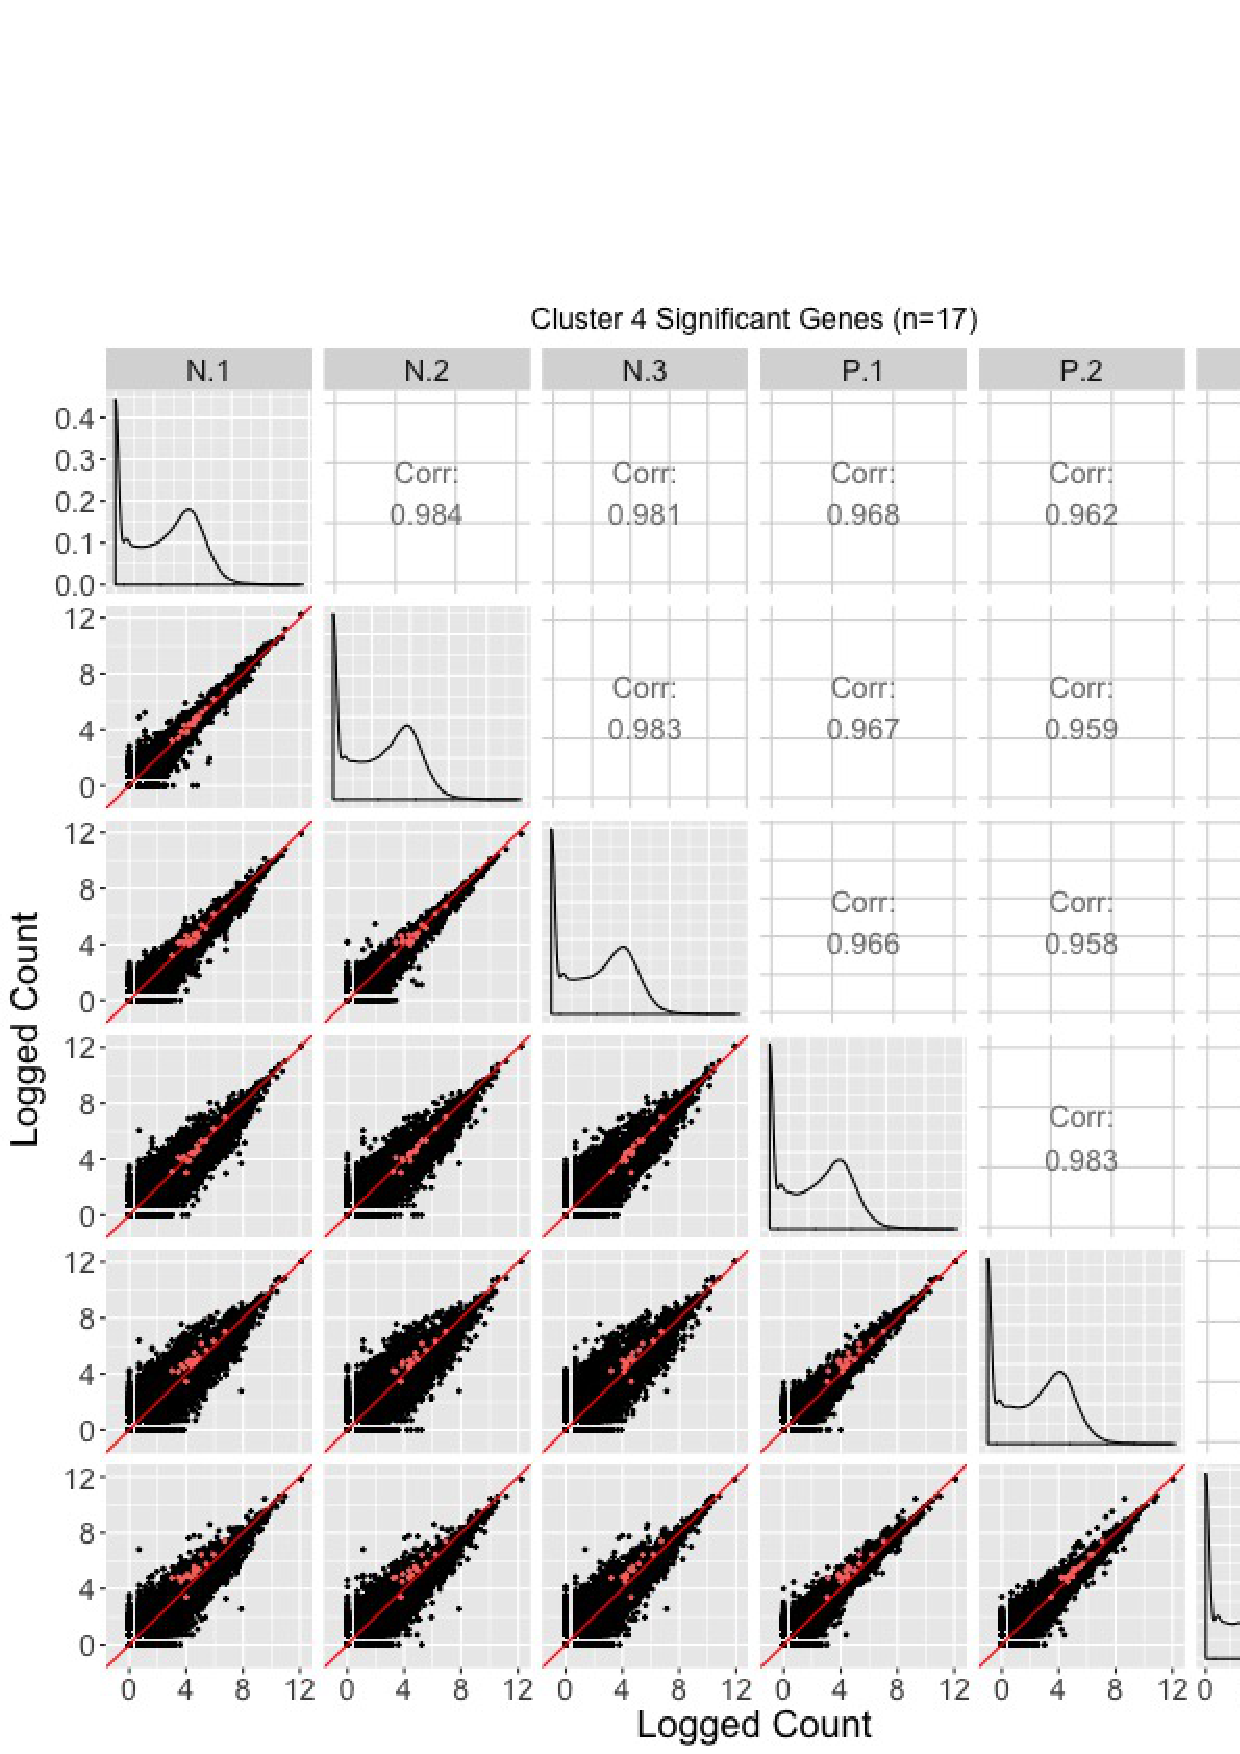
\includegraphics[width=\columnwidth]{../MakeFigures/sbIRClusterSigSM4.jpg}}
\caption{Example of using a scatterplot matrix to assess DEG calls from a model in the iron-metabolism soybean dataset. There were 17 significant genes in Cluster 4 after performing a hierarchical clustering analysis with a cluster size of four. These significant genes are overlaid in coral over the scatterplot matrix. For the most part, they do not seem to follow the expected patterns of differential expression: In many of the scatterplots between treatments, the coral points do not seem to deviate much from the \textit{x=y} line. Moreover, in the scatterplots between P.1 and P.2 as well as P.1 and P.3, the coral points seems to indicate an underexpression of the P.1 replicate. We found a similar finding of somewhat messy looking DEG calls in Cluster 4 from Figure 2 in the paper. 
\label{sbIRClusterSigSM4}}
\end{figure}  

\clearpage
\null
\begin{figure}[!t]
\centerline{\includegraphics[width=0.7\columnwidth]{../Bioinformatics/Pictures/mdsSwitch.png}}
\caption{Boxplots and MDS plots are popular plotting tools for RNA-seq analysis. This figure shows these traditional plots applied to the cotyledon data before sample switching (left half) and after sample switching (right half). We cannot suspect from the right boxplot that samples S1.3 and S2.1 have been swapped (subplots A). This is because all six samples have similar five number summaries. For the MDS plots, we do see a cleaner separation of the two treatment groups across the first dimension in the left plot than in the right plot (subplots B). However, taking into account the second dimension, both MDS plots contain three clusters, with sample S1.1 appearing in its own cluster. Without seeing one distinct cluster for each of the two treatment groups, it is difficult to suspect that samples S1.3 and S2.1 have been swapped in the right MDS plot (subplots B). We can only derive clear suspicion that the samples may have been switched by using plots that provide gene-level resolution like with the scatterplot matrix from Figure 6 in the main paper.
\label{mdsSwitch}}
\end{figure}

\clearpage
\null 
\begin{figure}[t!]
\centerline{\includegraphics[width=0.7\columnwidth]{../MakeFigures/Dashboards/litreCluster1/litreCluster1.jpg}}
\caption{Litre plots for significant genes inside Cluster 1 from Figure 2 of the paper. Subplots A and B each overlay a significant gene from Cluster 1 as nine green points. The genes show a pattern expected of a differentially-expressed one, by clumping together and deviating from the \textit{x=y} line. Moreover, the genes appear over-expressed in the P group. This is consistent with what we saw in Figure 2 of the paper. To interactively view the litre plot for all significant genes within Cluster 1, please visit https://rnaseqvisualization.shinyapps.io/litreCluster1.
\label{litreCluster1}}
\end{figure}   


\clearpage
The rest of the figures in this supplementary file (Figure~\ref{lkClustersKeep} through Figure~\ref{litreClusterAdd-St}) provide additional examples for the closing case study discussed in Section 5 of the main paper. In this case study, technical replicates of kidney and liver RNA-seq data was initially analyzed using library scale normalization. This process lead to 7,050 kidney DEGs and 1,968 liver DEGs, and visualization verification suggested that a subset of the kidney DEGs may be unreliable (Figure 10A from the main paper). Upon reviewing the geometrical structure of the data in the form of a scatterplot matrix, a subset of overexpressed liver genes was discovered, implicating the need for a more rigorous form of normalization (Figure 9 from the main paper). As a result, TMM normalization was then applied to the data, which lead to 3,974 kidney DEGs and 3,546 liver DEGs. These DEGs now appeared much more reliable (Figure 10B from the main paper). \\

In the remaining figures of this supplementary file, we thoroughly explore four subsets of genes from this case study in the form of parallel coordinate plots, scatterplot matrices, and litre plots. We also use variants of some of the techniques introduced in the main paper. Namely, we demonstrate the use of data standardization for scatterplot matrices and litre plots as a means to magnify the certain patterns at the expense of losing geometrical structure. In the below figures, we plot example genes from each of the four gene subsets using consistent color-coding. The four genes subsets and their color-codes are as follows:

\begin{itemize}

\item The 3,974 kidney DEGs from library scale normalization that remained as DEGs even after TMM normalization. These DEGs are plotted in \textbf{\textcolor{Fuchsia}{purple}}. As these genes were declared significant with both library scale normalization and TMM normalization, we expect them to follow the expected patterns of DEGs.

\item The 1,968 liver DEGs from library scale normalization that remained as DEGs even after TMM normalization. These DEGs are plotted in \textbf{\textcolor{Bittersweet}{orange}}. As these genes were declared significant with both library scale normalization and TMM normalization, we expect them to follow the expected patterns of DEGs.

\item The 3,076 kidney-specific DEGs from library scale normalization that were \textit{removed} as DEGs using TMM normalization. These DEGs are plotted in \textbf{\textcolor{Red}{red}}. As these genes were declared significant with library scale normalization but then removed as such with TMM normalization, we expect them to \textit{not} convincingly follow the expected patterns of DEGs.

\item The 1,578 liver-specific genes that were not detected as DEGs with library scale normalization but were then \textit{added} as such using TMM normalization. These DEGs are plotted in \textbf{\textcolor{RubineRed}{pink}}. As these genes were not declared significant with library scale normalization but were then declared as significant using the more-appropriate TMM normalization, we expect them to \textit{somewhat} convincingly follow the expected patterns of DEGs.

\end{itemize}

\noindent
The below figures are organized into five main groups as briefly explained below:

\begin{itemize}

\item Figure~\ref{lkClustersKeep} through Figure~\ref{lkClustersAdd} each shows the four gene subsets in the form of parallel coordinate plots after application of hierarchical clustering analysis. Each subset is grouped into eight clusters, not only to separate the genes into any subtle pattern differences, but also to reduce any overplotting that would occur should they all be viewed together as one large cluster. Overall, we see that the genes that were called DEGs in both forms of normalization (purple and orange) have very clean-looking parallel coordinate plots (especially in their largest cluster); the genes that were removed with TMM normalization (red) have messy-looking parallel coordinate plots; and the genes that were added with TMM normalization (pink) have decent-looking parallel coordinate plots.

\item Figure~\ref{lkClustersKeepSM} through Figure~\ref{lkClustersAddSM} each overlays the genes from the largest cluster of these four gene subsets in the form of scatterplot matrices. In general, we see that the genes that were called DEGs in both forms of normalization (purple and orange) have the expected profiles in the scatterplot matrices, deviating from the \textit{x=y} line in the treatment scatterplots in the anticipated direction. We also see that the genes that were removed with TMM normalization (red) do not show DEG patterns in the scatterplot matrices, as they barely deviate from the \textit{x=y} line in the treatment scatterplots. All three of these groups appear as predicted. However, perhaps surprisingly, the genes that were added with TMM normalization (pink) appear similarly to the genes that were removed with TMM normalization (red). We would expect the pink genes to deviate more from the \textit{x=y} line and demonstrate DEG patterns more than the red genes, but this was not observed.

\item Figure~\ref{litreClusterKeep} through Figure~\ref{litreClusterAdd} each overlays example genes from the largest cluster of these four gene subsets in the form of litre plots. Overall, we see that the example genes that were called DEGs in both forms of normalization (purple and orange) have the expected profiles in the litre plots, deviating in a concentrated bundle away from the \textit{x=y} line. We also see that the example genes that were removed with TMM normalization (red) do not show DEG patterns in the litre plots, barely deviating from the \textit{x=y} and/or being widely dispersed reflecting inconsistent replicates. All three of these groups appear as predicted. However, perhaps surprisingly, the genes that were added with TMM normalization (pink) appear similarly to the genes that were removed with TMM normalization (red). We would expect the pink genes to show DEG patterns (at least more than the red genes), but this was not observed.

\item Figure~\ref{lkClustersKeepSM-St} through Figure~\ref{lkClustersAddSM-St} are the same as Figure~\ref{lkClustersKeepSM} through Figure~\ref{lkClustersAddSM}, only now we \textit{standardized} the data. With standardization, we immediately note that the original geometric structure that elicited meaningful information about variation between treatments and replicates as well as the problematic streak of over-expressed liver genes is now gone. Instead, the dataset appears as an oval-shape that is almost identical across all scatterplots. However, in compensation for losing useful information in this sense, standardization appears to amplify other meaningful patterns. For instance, just as we saw in Figure~\ref{lkClustersKeepSM} through Figure~\ref{lkClustersAddSM}, the genes that were called DEGs in both forms of normalization (purple and orange) have the expected profiles. However, with standardization, we can see the replicates sticking to the \textit{x=y} line more clearly and we can also see which treatment group is expressed more clearly not only in the treatment scatterplots but also in the replicate scatterplots.

More importantly, while Figure~\ref{lkClustersKeepSM} through Figure~\ref{lkClustersAddSM} showed similar profiles for the genes that were added with TMM normalization (pink) and the genes that were removed with TMM normalization (red), standardization amplifies the differences between the pink and red gene profiles in a manner we would expect. Specifically, the standardized red gene profiles show widely dispersed genes that sometimes deviate from the \textit{x=y} line in the replicate scatterplots and cross both sides of and sometimes stick to the \textit{x=y} line in the treatment scatterplots. In other words, the red gene profiles often show patterns not akin to differential expression, as we would expect from these genes that were \textit{removed} as DEGs with TMM normalization. In contrast, the standardized pink gene profiles show less-widely dispersed genes that deviate less so from the \textit{x=y} line in the replicate scatterplots and deviate more from the \textit{x=y} line in the treatment scatterplots. In other words, the pink gene profiles show patterns more akin to differential expression than the red genes, as we would expect from these genes that were \textit{added} as DEGs with TMM normalization. At the same time, the pink gene profiles are not as clean-looking as the purple and orange genes that were designated as DEGs in both forms of normalization, which we might also expect. Overall, in these standardized scatterplot matrices, the pink genes appear as an intermediate between the clean-looking purple and orange genes and the messy-looking red genes.




\item Figure~\ref{litreClusterKeep-St} through Figure~\ref{litreClusterAdd-St} 

\end{itemize}


\clearpage
\null
\begin{figure}[t!]
\centerline{\includegraphics[width=0.65\columnwidth]{../MakeFigures/lkClustersKeep.jpg}}
\caption{Parallel coordinate plots showing hiearchical clustering analysis results of size eight for the 3,974 genes that remained in the kidney-specific DEGs after TMM normalization. We see that, for the most part, the parallel coordinate patterns follow the expected patterns across the clusters. The ideal pattern of DEGs is especially captured in the first cluster (the largest one with 1,136 genes). We used hierarchical clustering to mitigate additional overplotting that would occur if we were to plot all genes onto only one parallel coordinate plot.
\label{lkClustersKeep}}
\end{figure}

\null
\begin{figure}[t!]
\centerline{\includegraphics[width=0.65\columnwidth]{../MakeFigures/lkClustersOrig.jpg}}
\caption{Parallel coordinate plots showing hiearchical clustering analysis results of size eight for the 1,968 genes that were initially designated liver-specific DEGs after library scale normalization. We see that, for the most part, the parallel coordinate patterns follow the expected patterns across the clusters. The ideal pattern of DEGs is especially captured in the first cluster (the largest one with 933 genes). We used hierarchical clustering to mitigate additional overplotting that would occur if we were to plot all genes onto only one parallel coordinate plot.
\label{lkClustersOrig}}
\end{figure}

\null
\begin{figure}[t!]
\centerline{\includegraphics[width=0.65\columnwidth]{../MakeFigures/lkClustersRemove.jpg}}
\caption{Parallel coordinate plots showing hiearchical clustering analysis results of size eight for the 3,076 genes that were removed from the kidney-specific DEGs after TMM normalization. Unlike in Figure~\ref{KeepPCP}, the patterns in almost all clusters do not resemble the expected DEG format; instead, they show large variability between replicates and small variability between groups. In some clusters, it is difficult to even determine which group would be the overexpressed one if its genes were in fact DEGs. Taken together, this plot provides additional statistical evidence that the application of TMM normalization successfully removed genes that were previously mislabeled as kidney-specific DEGs (in Figure~\ref{RawKLSig}) with library scaling normalization. We used hierarchical clustering to mitigate additional overplotting that would occur if we were to plot all genes onto only one parallel coordinate plot.
\label{lkClustersRemove}}
\end{figure}

\null
\begin{figure}[t!]
\centerline{\includegraphics[width=0.65\columnwidth]{../MakeFigures/lkClustersAdd.jpg}}
\caption{Parallel coordinate plots showing hiearchical clustering analysis results of size eight for the 1,578 genes that were \textit{added} as liver-specific DEGs after TMM normalization. We see that, for the most part, the parallel coordinate patterns follow the expected patterns across the clusters. We used hierarchical clustering to mitigate additional overplotting that would occur if we were to plot all genes onto only one parallel coordinate plot.
\label{lkClustersAdd}}
\end{figure}

\null
\begin{figure}[t!]
\centerline{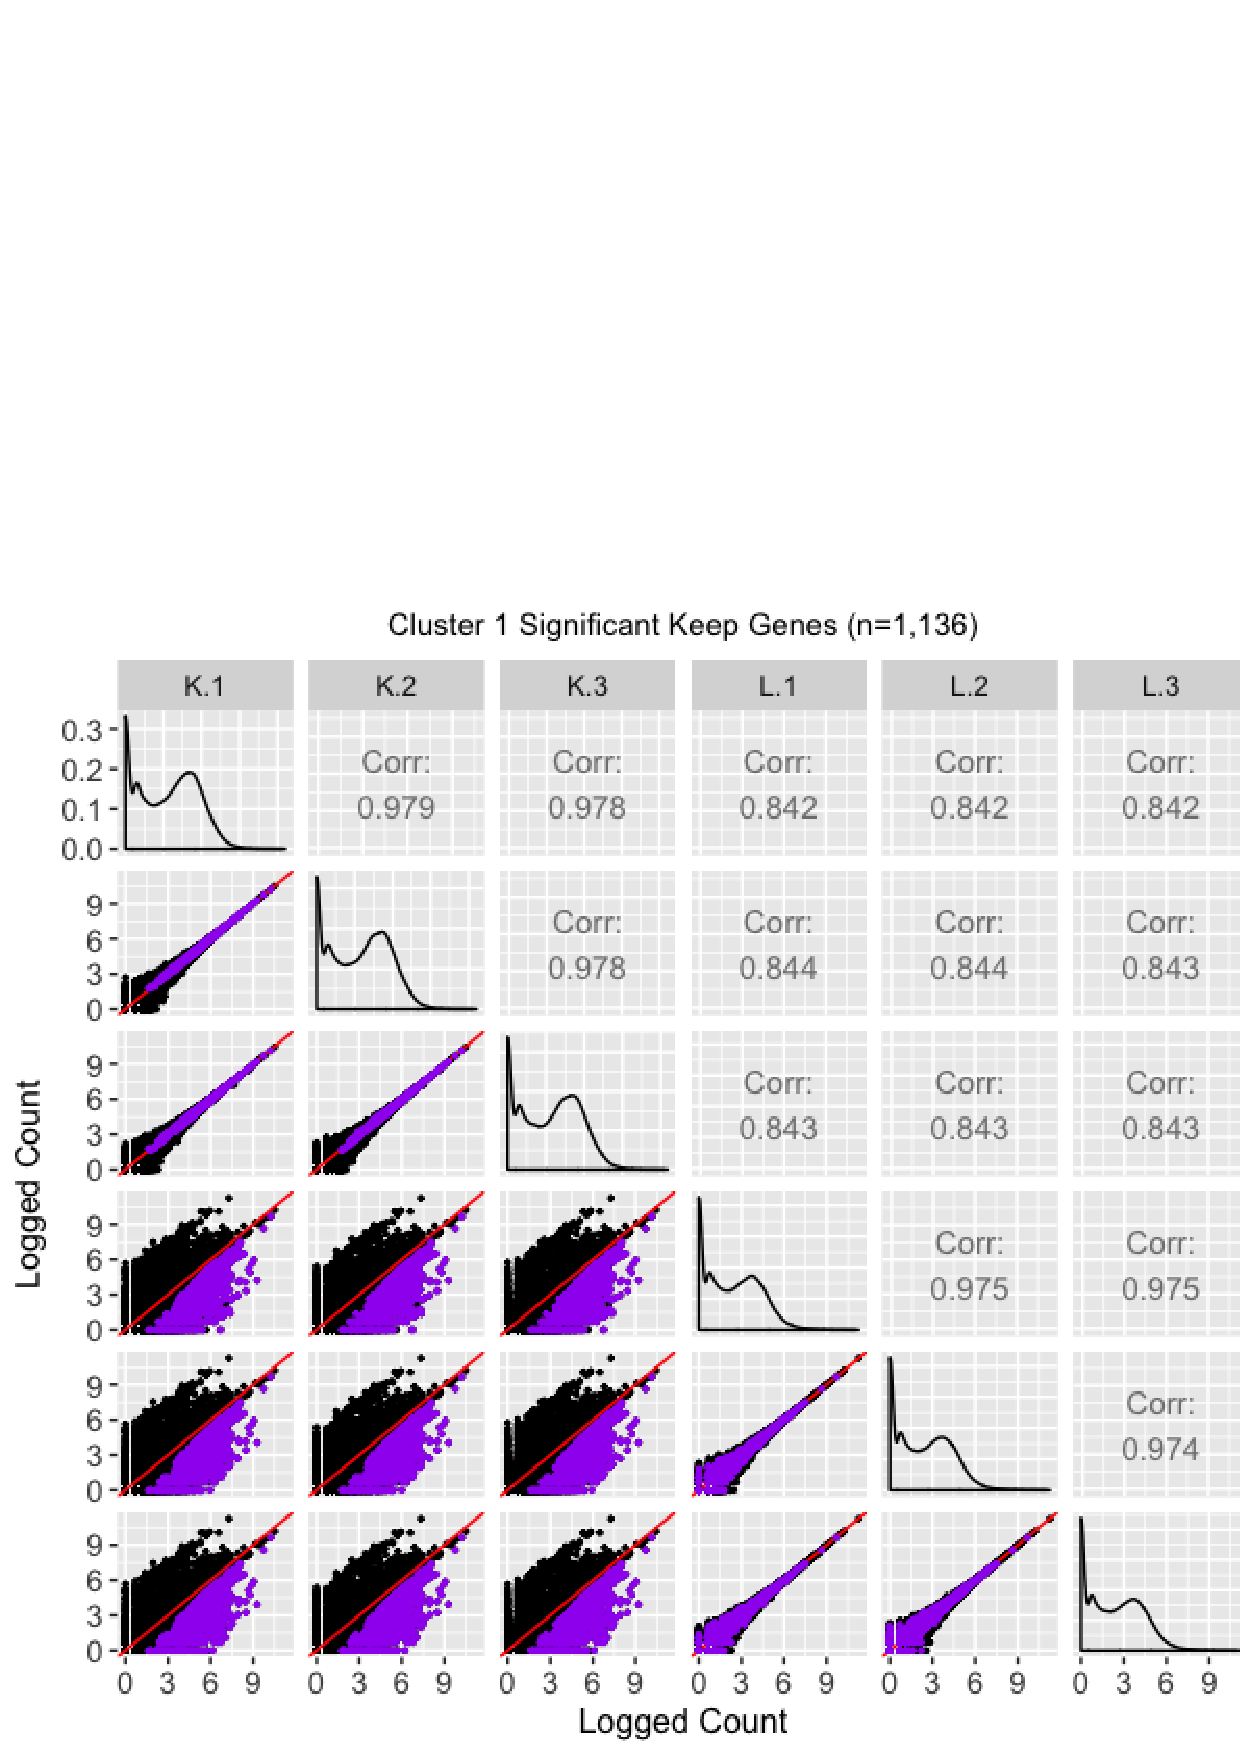
\includegraphics[width=1\columnwidth]{../MakeFigures/lkClustersKeepSM.jpg}}
\caption{Scatterplot matrix of the 1,136 genes that were in the first cluster (of Figure~\ref{lkClustersKeep}) from genes that remained as kidney-specific DEGs even after TMM normalization. With this scatterplot matrix, we verify from an additional perspective that these genes demonstrate the expected patterns of DEGs.
\label{lkClustersKeepSM}}
\end{figure}

\null
\begin{figure}[t!]
\centerline{\includegraphics[width=1\columnwidth]{../MakeFigures/lkClustersOrigSM.jpg}}
\caption{Scatterplot matrix of the 933 genes that were in the first cluster (of Figure~\ref{lkClustersOrig}) from genes that were initially designated as liver-specific DEGs after library scale normalization. With this scatterplot matrix, we verify from an additional perspective that these genes demonstrate the expected patterns of DEGs.
\label{lkClustersOrigSM}}
\end{figure}

\null
\begin{figure}[t!]
\centerline{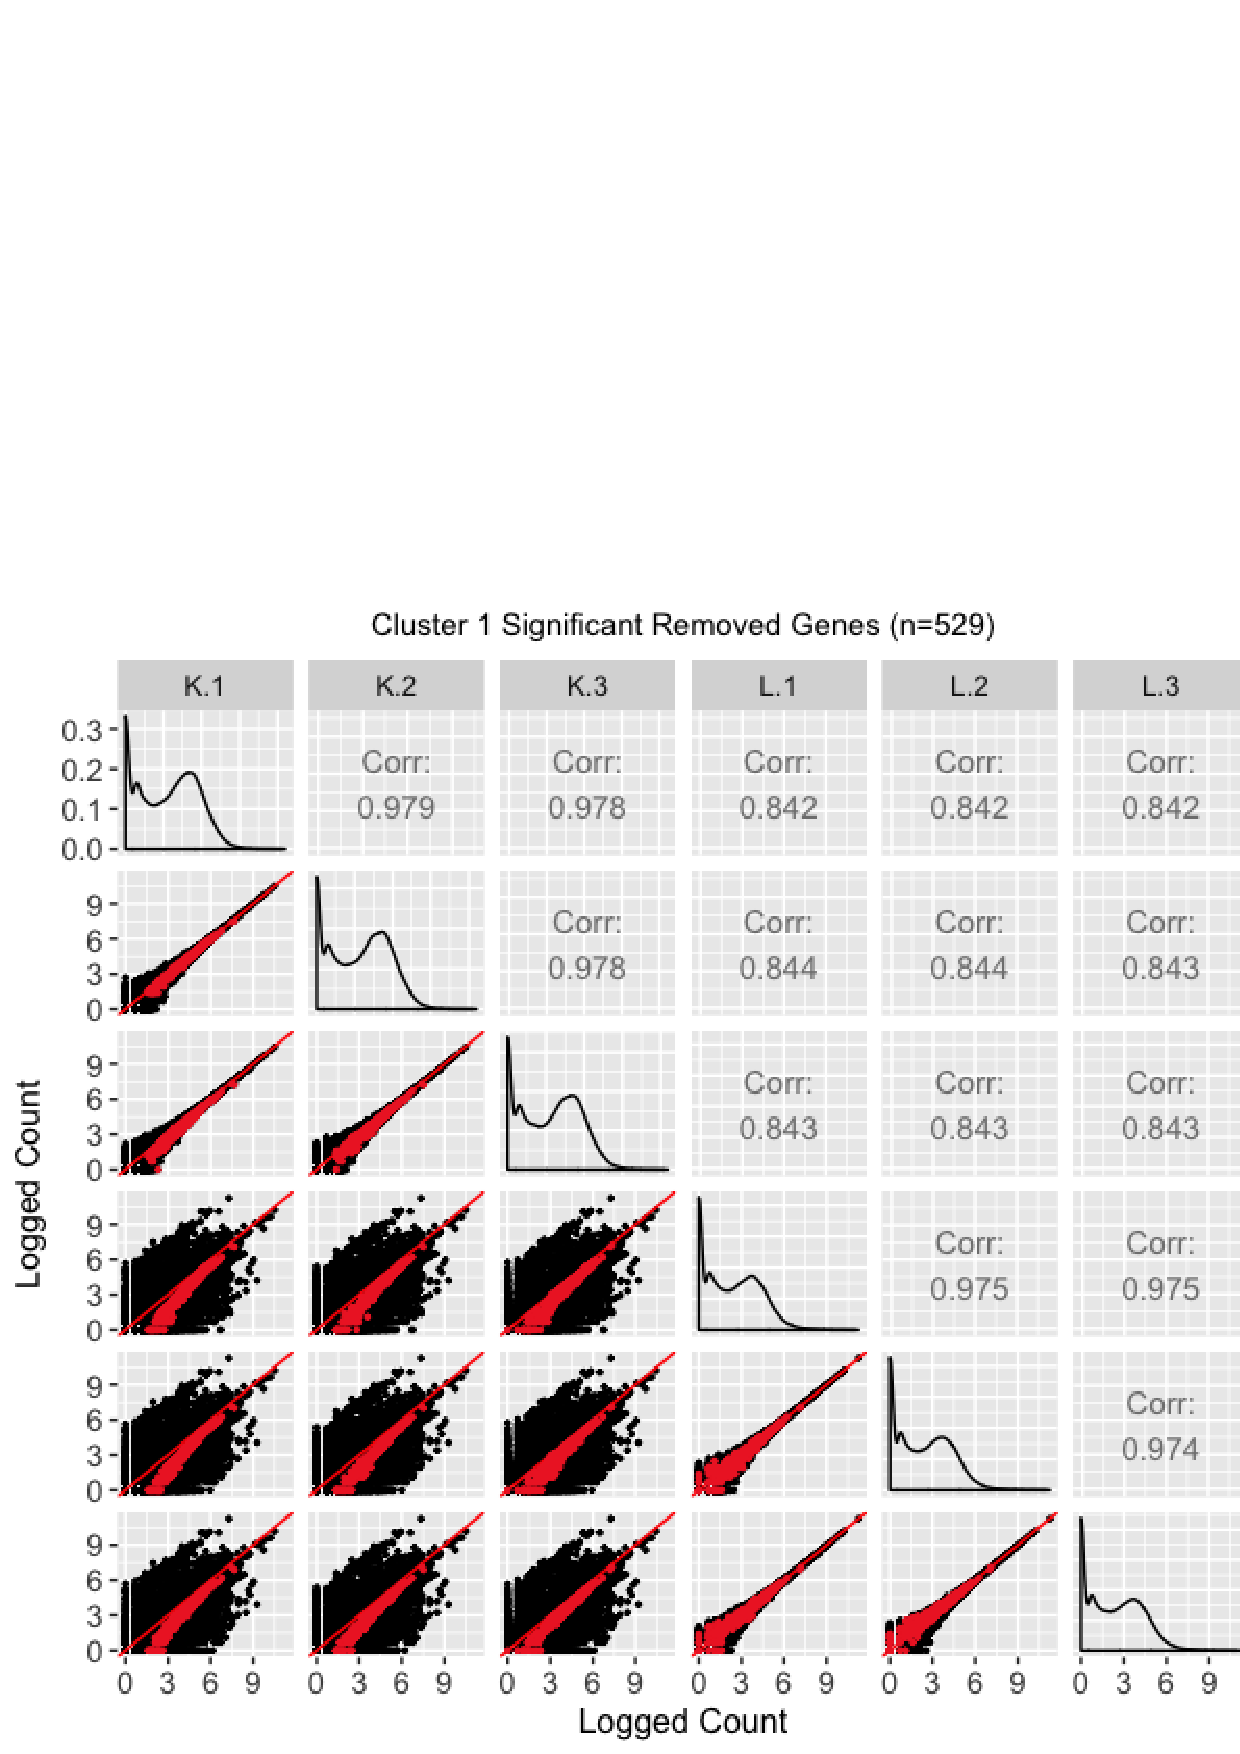
\includegraphics[width=1\columnwidth]{../MakeFigures/lkClustersRemoveSM.jpg}}
\caption{Scatterplot matrix of the 529 genes that were in the first cluster (of Figure~\ref{lkClustersRemove}) from genes that no longer remained as kidney-specific DEGs after TMM normalization. With this scatterplot matrix, we verify from an additional perspective that these genes do not demonstrate the expected patterns of DEGs too strongly (they do not deviate much from the \textit{x=y} line in the treatment scatterplots). This provides additional evidence that TMM normalization removing these genes from DEG status may be valid.
\label{lkClustersRemoveSM}}
\end{figure}

\null
\begin{figure}[t!]
\centerline{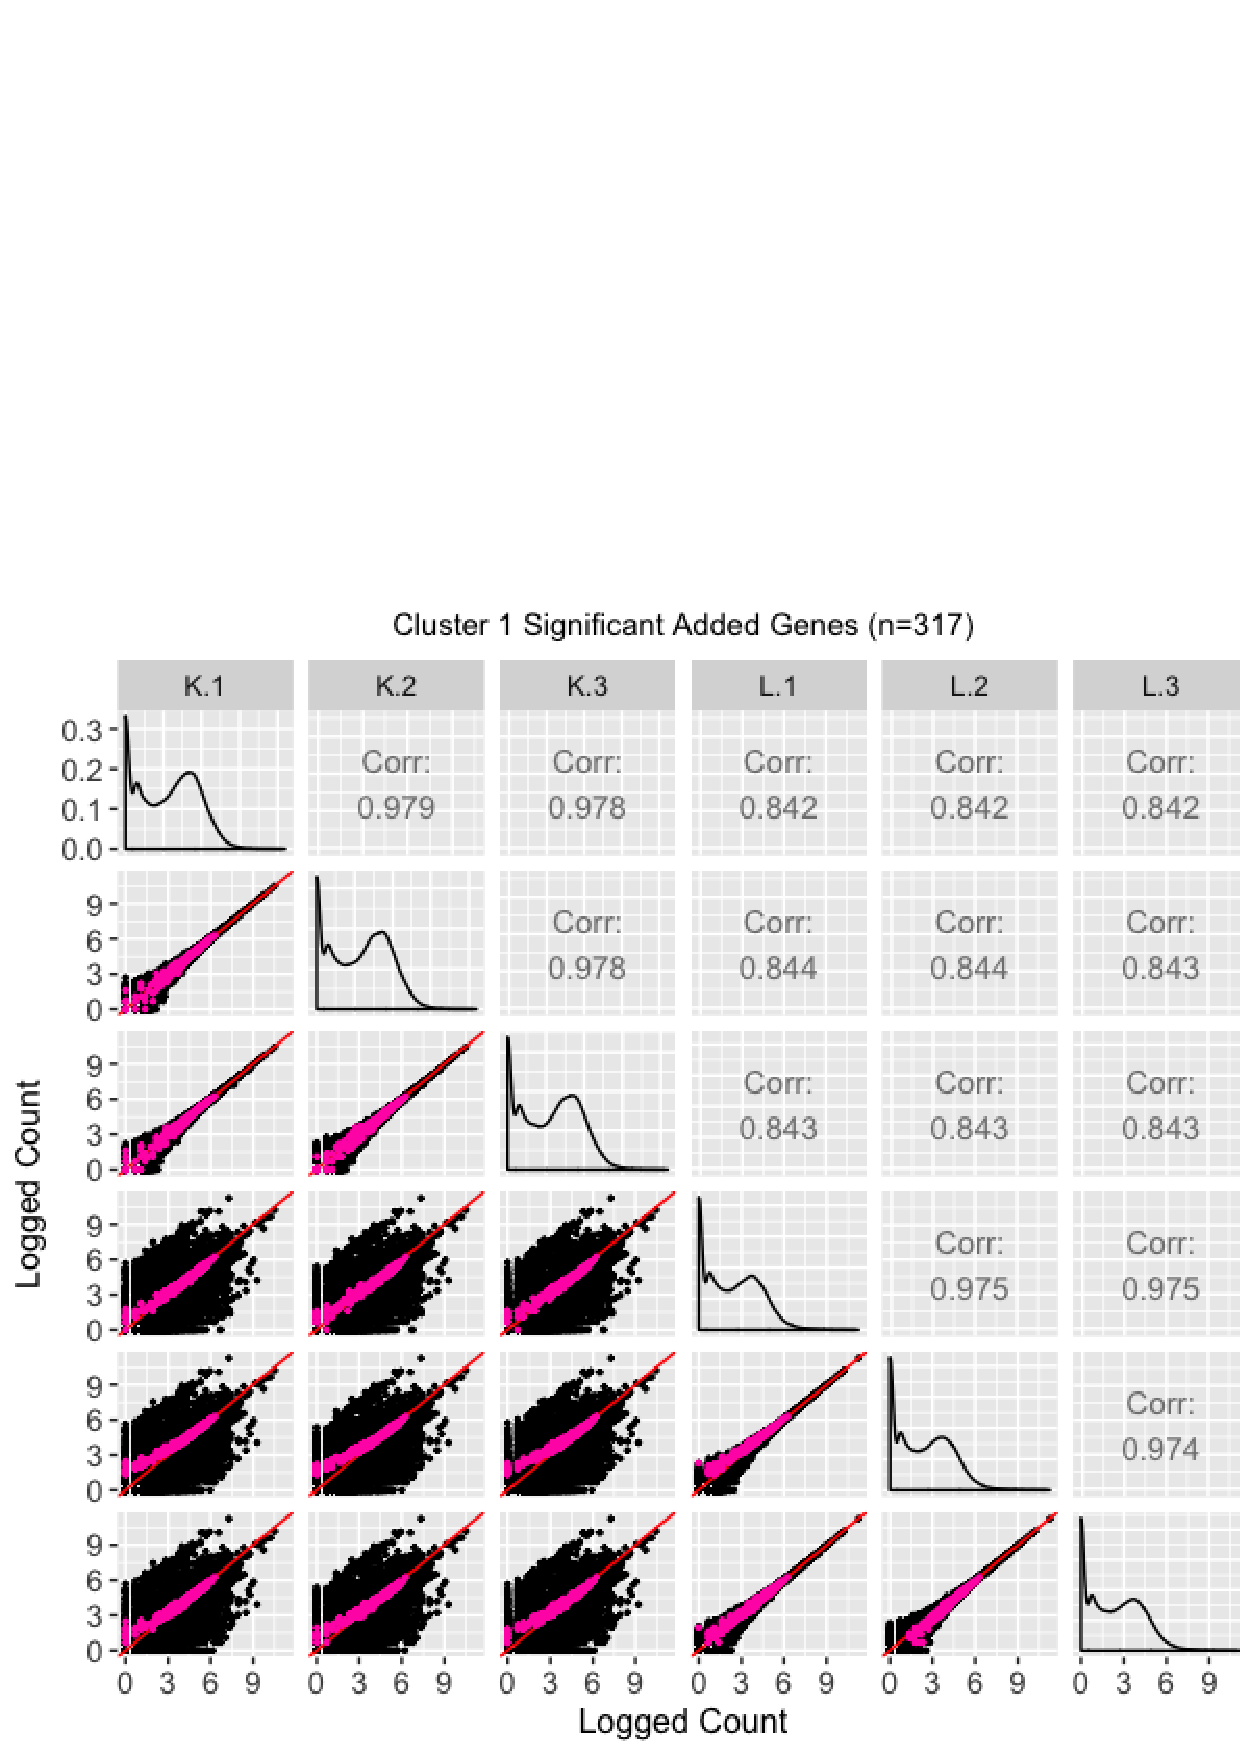
\includegraphics[width=1\columnwidth]{../MakeFigures/lkClustersAddSM.jpg}}
\caption{Scatterplot matrix of the 317 genes that were in the first cluster (of Figure~\ref{lkClustersAdd}) from genes that were \textit{added} as liver-specific DEGs after TMM normalization. With this scatterplot matrix, we are \textbf{unable} to verify from an additional perspective that these genes demonstrate the expected patterns of DEGs. (Need to find an explanation for this).
\label{lkClustersAddSM}}
\end{figure}


\null
\begin{figure}[t!]
\centerline{\includegraphics[width=0.7\columnwidth]{../MakeFigures/Dashboards/litreClusterKeep/litreClusterKeep.jpg}}
\caption{Example litre plots from the 1,136 genes that were in the first cluster (of Figure~\ref{lkClustersKeep}) of genes that remained kidney-specific DEGs even after TMM normalization. With these litre plots, we verify from an additional perspective that these genes demonstrate the expected patterns of DEGs.
\label{litreClusterKeep}}
\end{figure}

\null
\begin{figure}[t!]
\centerline{\includegraphics[width=0.7\columnwidth]{../MakeFigures/Dashboards/litreClusterOrig/litreClusterOrig.jpg}}
\caption{Example litre plots from the 933 genes that were in the first cluster (of Figure~\ref{lkClustersOrig}) from genes that were initially designated as liver-specific DEGs after library scale normalization. With these litre plots, we verify from an additional perspective that these genes demonstrate the expected patterns of DEGs.
\label{litreClusterOrig}}
\end{figure}

\null
\begin{figure}[t!]
\centerline{\includegraphics[width=0.7\columnwidth]{../MakeFigures/Dashboards/litreClusterRemove/litreClusterRemove.jpg}}
\caption{Example litre plots from the 529 genes that were in the first cluster (of Figure~\ref{lkClustersRemove}) of genes that no longer remained as kidney-specific DEGs after TMM normalization. With these litre plots, we verify from an additional perspective that these genes do not demonstrate the expected patterns of DEGs. This provides additional evidence that TMM normalization removing these genes from DEG status may be valid.
\label{litreClusterRemove}}
\end{figure}

\null
\begin{figure}[t!]
\centerline{\includegraphics[width=0.7\columnwidth]{../MakeFigures/Dashboards/litreClusterAdd/litreClusterAdd.jpg}}
\caption{Example litre plots from the 317 genes that were in the first cluster (of Figure~\ref{lkClustersAdd}) from genes that were \textit{added} as liver-specific DEGs after TMM normalization. With these litre plots, we are \textbf{unable} to verify from an additional perspective that these genes demonstrate the expected patterns of DEGs. (Need to find an explanation for this).
\label{litreClusterAdd}}
\end{figure}




\null
\begin{figure}[t!]
\centerline{\includegraphics[width=1\columnwidth]{../MakeFigures/lkClustersKeepSM-St.jpg}}
\caption{Scatterplot matrix of the \textit{standardized} 1,136 genes that were in the first cluster (of Figure~\ref{lkClustersKeep}) from genes that remained as kidney-specific DEGs even after TMM normalization. Even though the standardization process removes the interesting geometrical features we saw back in Figure~\ref{lkClustersKeepSM} regarding the streak of overexpressed liver genes, it allows us to view the DEG patterns in a more exaggerated fashion.
\label{lkClustersKeepSM-St}}
\end{figure}

\null
\begin{figure}[t!]
\centerline{\includegraphics[width=1\columnwidth]{../MakeFigures/lkClustersOrigSM-St.jpg}}
\caption{Scatterplot matrix of the \textit{standardized} 933 genes that were in the first cluster (of Figure~\ref{lkClustersOrig}) from genes that were initially designated as liver-specific DEGs after library scale normalization. Even though the standardization process removes the interesting geometrical features we saw back in Figure~\ref{lkClustersKeepSM} regarding the streak of overexpressed liver genes, it allows us to view the DEG patterns in a more exaggerated fashion.
\label{lkClustersOrigSM-St}}
\end{figure}

\null
\begin{figure}[t!]
\centerline{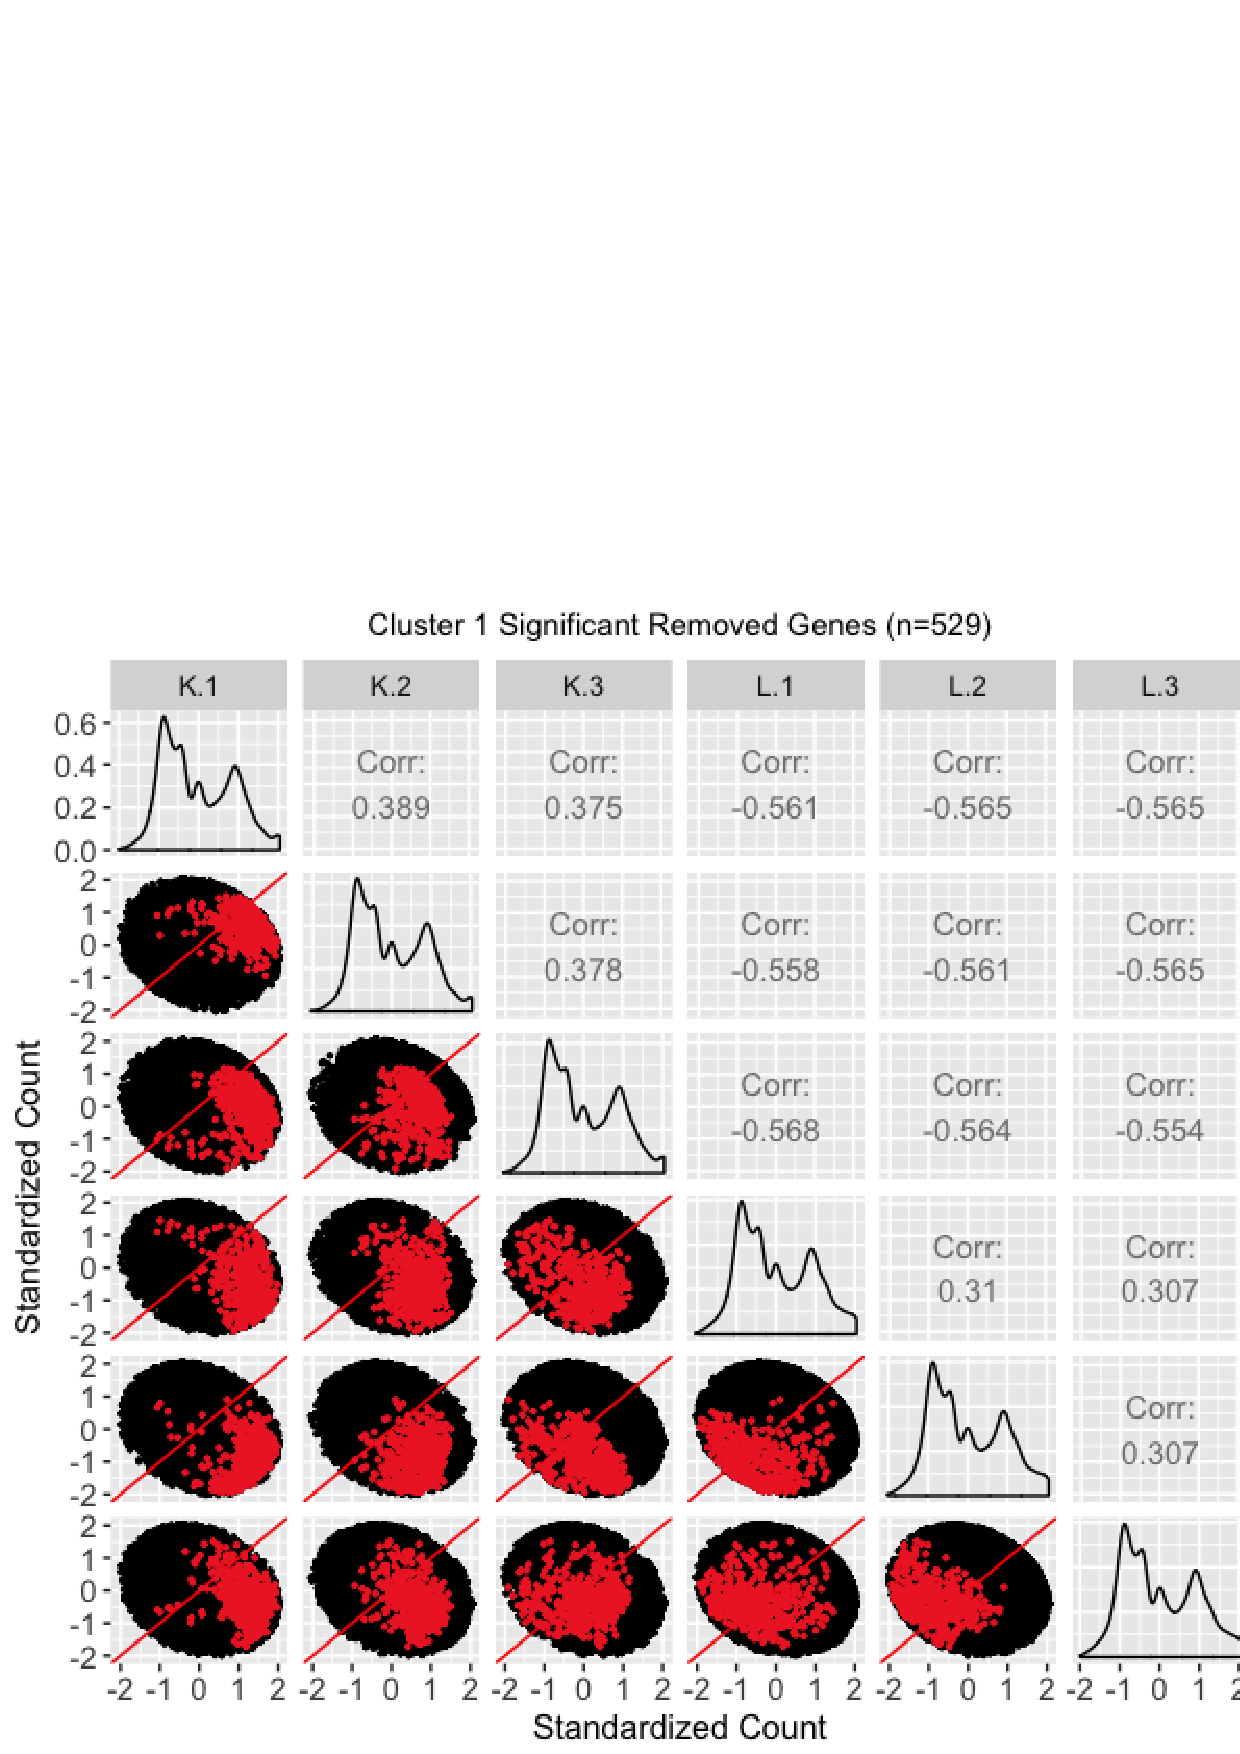
\includegraphics[width=1\columnwidth]{../MakeFigures/lkClustersRemoveSM-St.jpg}}
\caption{Scatterplot matrix of the \textit{standardized} 529 genes that were in the first cluster (of Figure~\ref{lkClustersRemove}) from genes that no longer remained as kidney-specific DEGs after TMM normalization. Even though the standardization process removes the interesting geometrical features we saw back in Figure~\ref{lkClustersKeepSM} regarding the streak of overexpressed liver genes, it allows us to view the DEG patterns in a more exaggerated fashion.
\label{lkClustersRemoveSM-St}}
\end{figure}

\null
\begin{figure}[t!]
\centerline{\includegraphics[width=1\columnwidth]{../MakeFigures/lkClustersAddSM-St.jpg}}
\caption{Scatterplot matrix of the \textit{standardized} 317 genes that were in the first cluster (of Figure~\ref{lkClustersAdd}) from genes that were \textit{added} as liver-specific DEGs after TMM normalization. Even though the standardization process removes the interesting geometrical features we saw back in Figure~\ref{lkClustersKeepSM} regarding the streak of overexpressed liver genes, it allows us to view the DEG patterns in a more exaggerated fashion.
\label{lkClustersAddSM-St}}
\end{figure}




\null
\begin{figure}[t!]
\centerline{\includegraphics[width=0.7\columnwidth]{../MakeFigures/Dashboards/litreClusterKeep-St/litreClusterKeep-St.jpg}}
\caption{Example litre plots from the 1,136 genes that were in the first cluster (of Figure~\ref{lkClustersKeep}) of genes that remained kidney-specific DEGs even after TMM normalization. With these litre plots, we verify from an additional perspective that these genes demonstrate the expected patterns of DEGs.
\label{litreClusterKeep-St}}
\end{figure}

\null
\begin{figure}[t!]
\centerline{\includegraphics[width=0.7\columnwidth]{../MakeFigures/Dashboards/litreClusterOrig-St/litreClusterOrig-St.jpg}}
\caption{Example litre plots from the 933 genes that were in the first cluster (of Figure~\ref{lkClustersOrig}) from genes that were initially designated as liver-specific DEGs after library scale normalization. With these litre plots, we verify from an additional perspective that these genes demonstrate the expected patterns of DEGs.
\label{litreClusterOrig-St}}
\end{figure}

\null
\begin{figure}[t!]
\centerline{\includegraphics[width=\columnwidth]{../MakeFigures/Dashboards/litreClusterRemove-St/litreClusterRemove-St.jpg}}
\caption{Example litre plots from the 529 genes that were in the first cluster (of Figure~\ref{lkClustersRemove}) of genes that no longer remained as kidney-specific DEGs after TMM normalization. With these litre plots, we verify from an additional perspective that these genes do not demonstrate the expected patterns of DEGs. This provides additional evidence that TMM normalization removing these genes from DEG status may be valid.
\label{litreClusterRemove-St}}
\end{figure}

\null
\begin{figure}[t!]
\centerline{\includegraphics[width=\columnwidth]{../MakeFigures/Dashboards/litreClusterAdd-St/litreClusterAdd-St.jpg}}
\caption{Example litre plots from the 317 genes that were in the first cluster (of Figure~\ref{lkClustersAdd}) from genes that were \textit{added} as liver-specific DEGs after TMM normalization. With these litre plots, we are \textbf{unable} to verify from an additional perspective that these genes demonstrate the expected patterns of DEGs. (Need to find an explanation for this).
\label{litreClusterAdd-St}}
\end{figure}




\end{document}